\chapter{Software}
El software es el elemento lógico que forma parte del ordenador, todo aquello que es “intangible”. Es el \textbf{conjunto de programas y datos} que permiten manejar el \hyperlink{hardware}{hardware}, controlando y coordinando su funcionamiento para que realice las tareas deseadas.

% para no copiar un trozo que ya tenemos en el fichero 1_introduccion.tex

\ExecuteMetaData[1_introduccion]{tipossoftware}


\section{Licencias de Software}
A la hora de utilizar cualquier tipo de software lo habitual es que tengamos que aceptar una licencia, que es un contrato entre el licenciante (autor o titular de los derechos de explotación y/o distribución del software) y el licenciatario (el usuario o consumidor final).

Las licencias incluyen una serie de términos y condiciones, que son un conjunto de permisos que el autor otorga al usuario.

{
    \begin{minipage}{0.4\linewidth}
        Algunos ejemplos de condiciones en una licencia pueden ser:
        \begin{itemize}
            \item Definir el tipo de uso.
            \item Limitar/permitir la distribución del software.
            \item Plazo de cesión de los derechos.
            \item Limitar/permitir la modificación del software.
        \end{itemize}
    \end{minipage}
    \hfill
    \begin{minipage}{0.55\linewidth}
%        \begin{center}
%            \vspace{-10pt}
            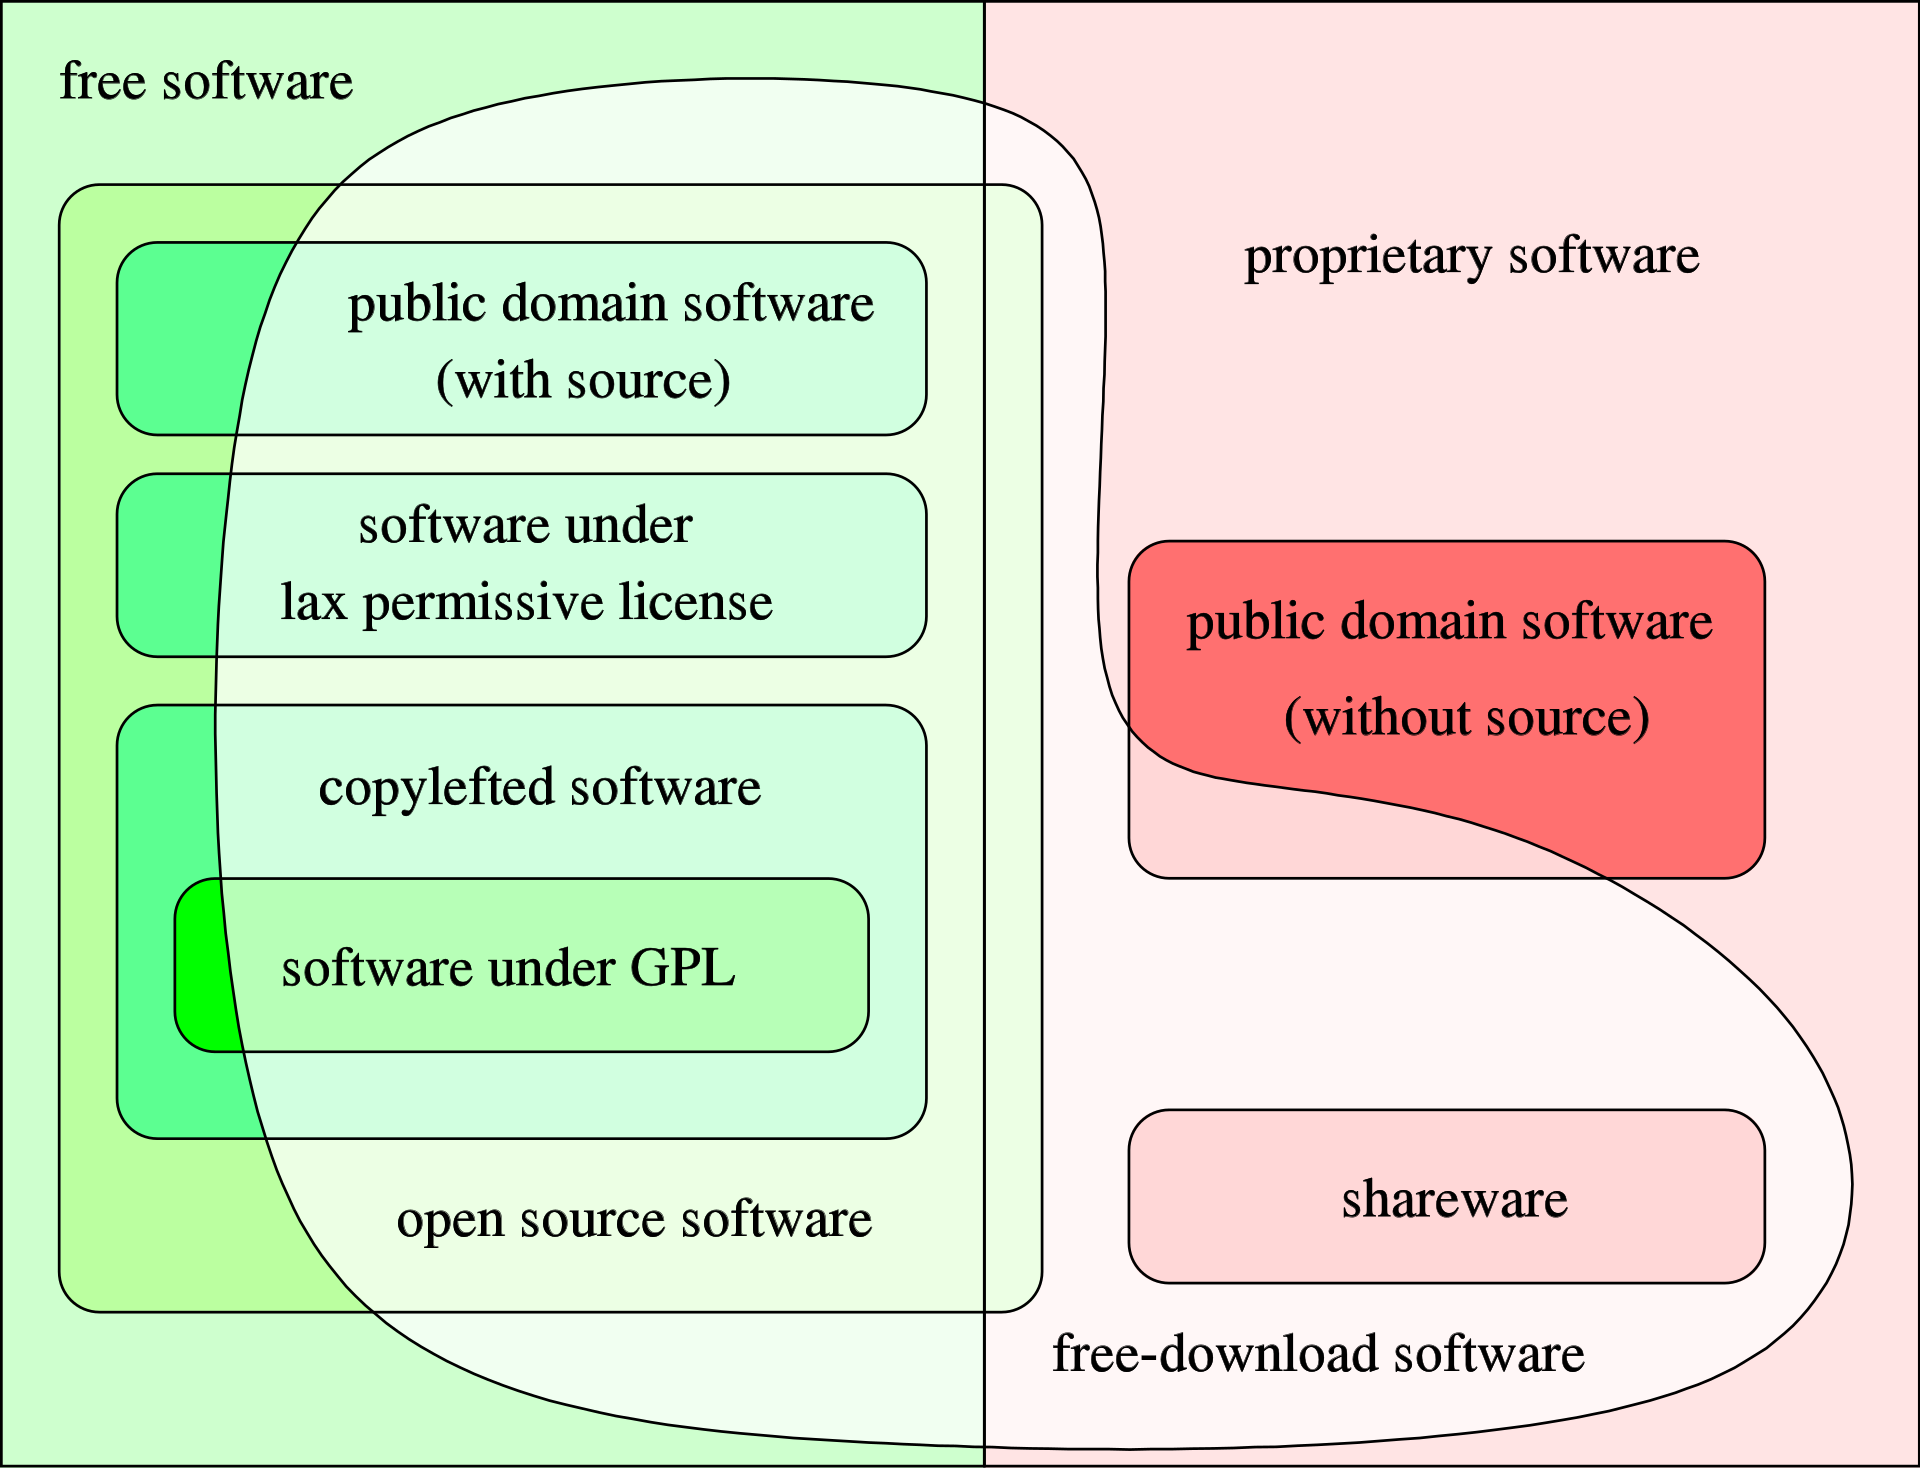
\includegraphics[width=\linewidth]{free_and_nonfree_software.png}
            \captionof{figure}{Esquema básico de licencias. Fuente: \href{https://en.wikipedia.org/wiki/Free_software\#Definition_and_the_Four_Essential_Freedoms_of_Free_Software}{Wikipedia}}
%        \end{center}
    \end{minipage}
}


% INCLUDE de sección de licencias libres
% modifico automáticamente secciones en subsecciones, y subsecciones en subsubsecciones

\let\foo\section %creo comando intermedio para luego recuperar cómo era la sección
\let\section\subsection
\let\subsection\subsubsection
% cambio el path de las imágenes
\graphicspath{{../../../temas_comunes/gnu_linux/img}}

\ExecuteMetaData[../../../temas_comunes/gnu_linux/gnu_linux]{softwarelibre}

%deshago todo lo hecho para la sección
\let\subsubsection\subsection
\let\subsection\section
\let\section\foo



\graphicspath{{img/si}}

% /INCLUDE

\subsection{Software privativo}
En contraposición al Software Libre se encuentra el software privativo, el cuál \textbf{no permite} el acceso al código fuente, ya que sólo se encuentra a disposición de los desarrolladores, no permitiendo su libre modificación, adaptación o distribución.

Dentro de este tipo de software podemos encontrar algunos tipos de licenciamiento conocidos:

\begin{itemize}
    \item \textbf{Freeware}: Normalmente se utiliza para el software que es gratuito pero que no permite la modificación del mismo.
    \item \textbf{Shareware}: El usuario puede evaluar de forma gratuita el producto, durante un tiempo limitado o con una funcionalidad limitada.
\end{itemize}

Entre el software más utilizado que es software privativo nos podemos encontrar a: Windows, Photoshop, juegos comerciales, ...

\subsection{Software de dominio público}
Es aquel que el autor decide publicarlo bajo el denominado \href{https://es.wikipedia.org/wiki/Dominio_p%C3%BAblico}{dominio público}, lo que hace que cualquiera pueda acceder al código fuente, modificarlo \textbf{pero también publicarlo bajo una licencia no libre}.

Este tipo de licencia suele ser aplicada a libros y música, por ejemplo, tras 70 años después de la muerte del autor.



\chapter{Sistemas Operativos}

El Sistema Operativo (\textbf{SO}) es el \textit{software} que controla el \textit{hardware} del ordenador, creando recursos lógicos y servicios que otro software y los usuarios pueden utilizar.

De manera muy simplificada, el núcleo del Sistema Operativo crea una abstracción del hardware real, limitando el acceso al mismo a los programas para gestionar su buen funcionamiento.

\section{Funciones principales}

Entre las funciones más importantes de las que se encarga el Sistema Operativo, destacaremos:

\begin{itemize}
    \item \textbf{Gestionar los procesos en ejecución}: El sistema operativo se encarga de cargar el proceso que queramos ejecutar y de asignarle los recursos necesarios para su correcto funcionamiento. También se encarga de las posibles peticiones de los procesos, de pausarlos, de asignarles el procesador cuando le corresponda...

    \item \textbf{Gestionar la memoria RAM}: La memoria RAM es finita en el ordenador, y cuando ejecutamos un proceso este se carga en RAM para poder ser ejecutado. Si un proceso necesitase más memoria, será el sistema operativo el que se encargue de asignarle más en caso de que haya libre. Cuando los procesos mueren, esa memoria debe ser liberada, para que otros procesos puedan utilizarla.

    \item \textbf{Administrar la CPU} gracias a un algoritmo de programación: El sistema operativo coordina el uso de la CPU entre las diferentes tareas y procesos que se ejecutan en el sistema. Utiliza algoritmos de programación para determinar el orden y la prioridad de ejecución de los procesos, asegurando un uso equitativo de los recursos de la CPU.

    \item \textbf{Gestionar las entradas y salidas} de datos a través de los periféricos: Además de direccionar las entradas y salidas de datos, el sistema operativo proporciona controladores (\textbf{\textit{drivers}}) para interactuar con los periféricos de entrada y salida, como teclados, mouse, impresoras, discos duros externos, entre otros. Estos controladores permiten que los dispositivos se comuniquen correctamente con el sistema operativo y las aplicaciones.

    \item \textbf{Asegurar el buen funcionamiento del sistema}: El sistema operativo gestiona información esencial para el funcionamiento del sistema, como la tabla de procesos, la tabla de archivos abiertos y otros datos relevantes. Además, realiza la gestión del rendimiento para asegurar un funcionamiento óptimo del sistema.

    \item \textbf{Seguridad}: El sistema operativo proporciona un mecanismo de autenticación y autorización para garantizar que los usuarios accedan solo a los recursos y funciones para los cuales tienen permisos. Esto incluye la gestión de cuentas de usuario, contraseñas y asignación de privilegios.

    \item \textbf{Administrar los archivos}: El sistema operativo maneja las operaciones relacionadas con la gestión de archivos, como la creación, modificación, eliminación y acceso a los archivos en el sistema de almacenamiento.
\end{itemize}


\section{Breve historia de los sistemas operativos}

Desde la creación de los primeros ordenadores, y al igual que ha sucedido con estos, los sistemas operativos han sufrido una evolución. A continuación un breve repaso, pudiendo ver toda la información en  \href{https://es.wikipedia.org/wiki/Historia_de_los_sistemas_operativos}{Wikipedia}.

\begin{itemize}
    \item \textbf{Sin sistema operativo}: Los primeros ordenadores no contaban con un sistema operativo propio. Los ordenadores electromecánicos sólo podían ejecutar el programa para el que fueron construidos.

    Con la aparición de los primeros ordenadores digitales, se programaban en lenguaje máquina y ejecutaban el programa. En caso de querer ejecutar otro programa, había que cargarle el programa a mano.

    \item \textbf{Sistemas Batch}: A principios de los años 1950 aparecen los “monitor residente” que se encargan de cargar los programas leyéndolos de tarjetas perforadas o de cintas para su posterior ejecución.

    \item \textbf{Sistemas “multiprogramados” y tiempo compartido}: En la década de 1960, aparecen los sistemas operativos que son capaces de ejecutar procesos de un programa mientras otro está a la espera de una operación de E/S.

    También aparecen los sistemas multiusuario, y el “\textit{scheduling}” del sistema, que lo que hace es compartir tiempo de ejecución del procesador entre distintos programas, dándoles un tiempo a cada uno.

    A principios de 1970 se crea Unix, un sistema operativo muy importante en la época y del cuál han salido variaciones que siguen hoy en día usándose.

    \item \textbf{Sistemas en red}: Con la aparición de las redes de ordenadores, empiezan a aparecer sistemas operativos con acceso a la red y ofreciendo servicios que pueden ser utilizados por usuarios o por otros ordenadores.

    \item \textbf{Sistemas operativos de escritorio}: En la década de 1980, con la aparición y proliferación de ordenadores personales (PC), empiezan a aparecer sistemas operativos más enfocados a usuarios que no son expertos en informática.

    Aparecen los primeros interfaces de usuario y escritorios (primero con el Macintosh de Apple en 1984) que junto al ratón facilita la usabilidad de los programas.
\end{itemize}







%    \section{Tipos de Software}
%    \subsection{firmware,sistema y aplicaciones}
%
%
%